\begin{frame}{Propensity Score Issues}
 \begin{itemize}
  \item Unmeasured confounders
  \item Choice of pretreatment covariates in the propensity score model
  \item Different models and methods may lead to different conclusions
 \end{itemize}

\end{frame}

\begin{frame}{Joint Modelling (JM)}
 \begin{itemize}
  \item Assume ignorable MAR  missing data mechanism
  \item Missing data imputed by sampling from a user specified distribution
  \item A lot of theory developed for Normal, not much else
  \begin{itemize}
   \item Normal imputation has been shown to perform well, even under non normality \cite{Demirtas2008}
  \end{itemize}
\item Idea: pull imputations by missing data row pattern
 \end{itemize}

\end{frame}

\begin{frame}{JM pseudocode}
 \begin{figure}[h!]
  \centering
    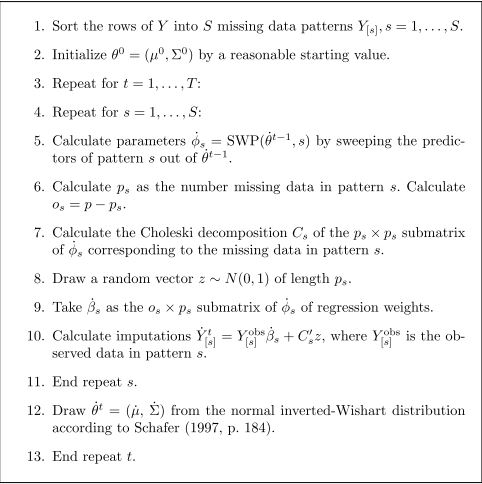
\includegraphics[width=0.6\textwidth]{jm_algo}
 % \caption{Normal JM imputation pseudocode}
\label{fig:jmexample}
\end{figure}
%do I want to include the amelia algo?
\end{frame}

\begin{frame}{JM Pros and Cons}
Pros
 \begin{itemize}
  \item Fast
  \item Easy to derive posteriors with common distributions
 \end{itemize}

 Cons
 \begin{itemize}
  \item Inflexible
  \item Limited to known distributions
  \item How to deal with mixed categorical and continuous missing data
 \end{itemize}

\end{frame}
